
\chapter{Introduzione al campionamento}


\section{Introduzione}
L'esame di un campione comprende sia l'analisi macroscopica che quella microscopica. Tra le due, quest'ultima è indubbiamente la più apprezzata, forse perché esteticamente più piacevole, priva di odori particolari e non richiede alcuno sforzo manuale se non lo spostamento del vetrino sotto il microscopio, mantenendolo a fuoco e cambiando gli obiettivi. Più piccolo è il campione, meno significativa appare l'analisi macroscopica. Alcuni la vedono solo come un passaggio tecnico, paragonabile alla preparazione dei tessuti. Alcuni colleghi hanno addirittura affermato che la patologia autoptica è patologia macroscopica, mentre la patologia chirurgica è istopatologia.

\subsection{L'importanza dell'esame macroscopico}
È spiacevole che questo atteggiamento sia così diffuso tra i patologi. Come ha affermato Chandler Smith nel suo saggio "In lode dell'esame macroscopico", è proprio l'aspetto macroscopico che rivela le dimensioni, la forma e la natura del processo, consentendo una comprensione sia strutturale che clinica. In alcuni campioni, come le valvole cardiache, un attento esame macroscopico e una descrizione accurata forniscono molte più informazioni rispetto a una sezione microscopica casuale. In molti casi, una dissezione macroscopica inadeguata può compromettere l'interpretazione microscopica.

\subsection{La dissezione come fase cruciale}
La dissezione, la descrizione macroscopica e la selezione delle sezioni per lo studio microscopico sono una parte cruciale dell'esame patologico. Se la descrizione microscopica è inadeguata, il vetrino può essere riesaminato e il problema corretto. Tuttavia, se non vengono registrate le dimensioni del campione, non vengono prelevate sezioni chiave o non vengono eseguiti studi speciali durante l'esame macroscopico iniziale, c'è il rischio che queste informazioni vadano perse per sempre.

\subsection{L'esperienza è fondamentale per campioni complessi}
I campioni complessi richiedono esperienza e conoscenza per essere adeguatamente sezionati, descritti e campionati. Esiste una curiosa reticenza tra i medici in formazione e i giovani patologi nel consultare un membro senior del personale per il corretto trattamento di campioni macroscopici difficili, mentre lo stesso freno non si osserva quando devono affrontare una sezione microscopica complicata. Questo è un peccato, poiché a volte la difficoltà di interpretazione del vetrino deriva da un campionamento macroscopico inadeguato.

\section{Dall'accettazione alla processazione}

\subsection{Posizione ideale del laboratorio}
La disposizione ottimale prevede che il laboratorio di anatomia patologica sia in stretta prossimità della sala operatoria. I campioni, eccetto piccole biopsie, dovrebbero essere inviati al laboratorio in uno stato fresco e trasportati immediatamente dopo la resezione in un sacchetto di plastica senza contenitori rigidi o metallici. È importante evitare il contatto con liquidi che potrebbero compromettere la conservazione del campione. Se si prevede un ritardo nel trasporto al laboratorio, è consigliabile refrigerare il campione per rallentare il processo autolitico.


\subsection{Trattamento delle biopsie}
Le biopsie di piccole dimensioni, comprese biopsie endoscopiche, biopsie incisionale e microscopiche, devono essere immediatamente collocate nel fissativo scelto subito dopo essere state ottenute. Per i campioni di medie o grandi dimensioni che richiedono un trasporto più lungo, si è proposto un compromesso interessante: sigillare il campione in un sacchetto di plastica sotto vuoto. Tuttavia, questo metodo presenta il rischio che l'operatore creda erroneamente che il campione sia già in fase di fissazione, il che potrebbe non essere vero.


\subsection{La preparazione e la dissezione dei campioni}
La dissezione e la preparazione di un campione per l'analisi istologica e microscopica comprendono molto più che il semplice processamento del tessuto e il taglio delle sezioni. Anche se la dissezione e l'area di laboratorio sono spesso considerate gli elementi chiave del dipartimento, è essenziale comprendere che ci sono molti altri passaggi che seguono la ricezione del campione. Alcuni di questi sono specifici per la selezione e la manipolazione dei tessuti, mentre altri svolgono chiaramente un ruolo di supporto. È implicito, inoltre, che un buon laboratorio sia dotato di personale scientifico/medico adeguatamente formato e di personale di supporto, poiché interagiscono a più livelli con la gestione dei campioni patologici. Infatti, un dipartimento con personale insufficiente fornirà inevitabilmente prestazioni deboli, nella migliore delle ipotesi.

\subsection{La stanza dell'accettazione}
Un locale separato è necessario per la ricezione dei campioni, fungendo da interfaccia tra il personale ospedaliero (o altri visitatori) e il  campionamento. Devono essere presenti piani di lavoro adeguati e una buona illuminazione, insieme a una buona ventilazione, attrezzature di sicurezza, disinfettanti, granuli assorbenti e indumenti protettivi. In caso di fuoriuscita di campioni, come liquidi corporei o perdite di fissativi, la risposta immediata del personale limiterà qualsiasi potenziale rischio per la salute e preverrà rischi per gli altri operatori di laboratorio.

\subsection{L'accettazione del campione}
Il punto centrale di questa stanza è ricevere i campioni in modo sicuro e protetto. Il campione deve essere identificato e gli deve essere assegnato un identificatore unico di laboratorio, generalmente un numero complesso. È obbligatorio confrontare il campione con il modulo di richiesta clinica e verificare i dettagli clinici appropriati. Dati corroborativi come il numero di registrazione ospedaliera, il codice fiscale del paziente, il nome completo, la data di nascita e l'indirizzo sono metodi validi per verificare l'identità di un campione. Se vi è qualche dubbio sull'integrità del campione, non dovrebbe essere inoltrato fino a quando il medico responsabile non abbia confermato i dettagli appropriati.

\subsection{Regole per la verifica del campione}
In molte situazioni è preferibile seguire la regola del "doppio controllo", con due operatori indipendenti che verificano i vari dettagli del campione in tutte le fasi dell'esame. È consigliabile confermare almeno tre identificatori univoci del campione. Una volta convalidato e identificato, il caso può essere trasferito alla sala di dissezione per l'esame, la descrizione del campione e la campionatura per blocchi.

\subsection{Il numero istologico}
Il metodo più comune di identificazione del campione è l'anno (spesso espresso con due cifre) con un sistema di numerazione sequenziale che parte da uno (1) e procede fino all'ultimo campione dell'anno. Questo sistema semplice permette di processare con facilità i campioni di patologia chirurgica e di correlare i blocchi di paraffina, le fotografie e altri test associati.



\subsection{Valutazione iniziale dei campioni}
I campioni ricevuti nel laboratorio devono essere esaminati non appena possibile, sulla base delle informazioni cliniche disponibili e delle caratteristiche macroscopiche. Questo permette di determinare se siano necessari ulteriori esami, come sezioni congelate o altri esami specifici oltre alla valutazione macroscopica e microscopica di routine.

\subsection{Procedure speciali}
Esistono diverse procedure speciali da applicare in base alle caratteristiche del campione:
\begin{itemize}
    \item Colture batteriche, fungine e virali
    \item Microscopio elettronico
    \item Colorazioni istochimiche e immunoistochimiche
    \item Preparazioni citogenetiche
    \item Studi di genetica molecolare
    \item Fotografie convenzionali o digitali
    \item Inclusioni in resina plastica per sezioni sottili (1 $\mu$m)
    \item Radiografie
    \item Fissativi speciali (diversi dalla formalina di routine)
    \item Colture cellulari
    \item Necessità per la banca dei tumori
\end{itemize}


\subsection{Ruolo dei \textit{Pathologists' Assistants}}
È estremamente utile disporre di un team di "assistenti del patologo" appositamente formati per eseguire gli aspetti tecnici di questi studi in modo coerente, sotto la direzione e supervisione del patologo. Questi assistenti dovrebbero essere competenti nella fotografia macroscopica, tecniche radiografiche, iniezione di campioni, taglio e colorazione per sezioni congelate e altre mansioni tecniche svolte nella sala macroscopica. La presenza di questi collaboratori consente non solo di liberare il patologo per altre attività, ma garantisce anche una coerenza nell'esecuzione dei test che altrimenti sarebbe difficile da ottenere.


\subsection{La dissezione e il taglio del campione}
La disposizione ideale della sala di dissezione varia tra i laboratori e le esigenze dei patologi. Esistono diverse soluzioni di design che si basano sui principi generali di un laboratorio di istologia. Tuttavia, è imperativo che l'area di dissezione abbia una buona illuminazione, ventilazione, superfici non assorbenti e facili da pulire, insieme a indumenti protettivi appropriati, guanti e altre attrezzature come macchine fotografiche, lavandini con tritarifiuti e contenitori per lo smaltimento dei rifiuti. La sala di dissezione dovrebbe essere un ambiente protetto che permetta al patologo e al personale tecnico di lavorare senza disturbi.

\section{Caratteristiche Generali della Sala Macroscopica}
Le dimensioni e le caratteristiche della sala macroscopica di patologia chirurgica dipendono dal numero di campioni, dal numero di patologi e medici in formazione, e dal tipo di istituzione. La sala descritta nei paragrafi seguenti è modellata su un grande laboratorio in un'istituzione accademica, ma molti dei requisiti si applicano anche ai laboratori di piccoli ospedali.

\subsection{Dimensioni e Illuminazione}
Prima di tutto, la sala dovrebbe essere abbastanza spaziosa da permettere a tutti i patologi assegnati alle attività macroscopiche di lavorare simultaneamente; deve essere ben illuminata e correttamente ventilata.

\begin{figure}[h]
    \centering
    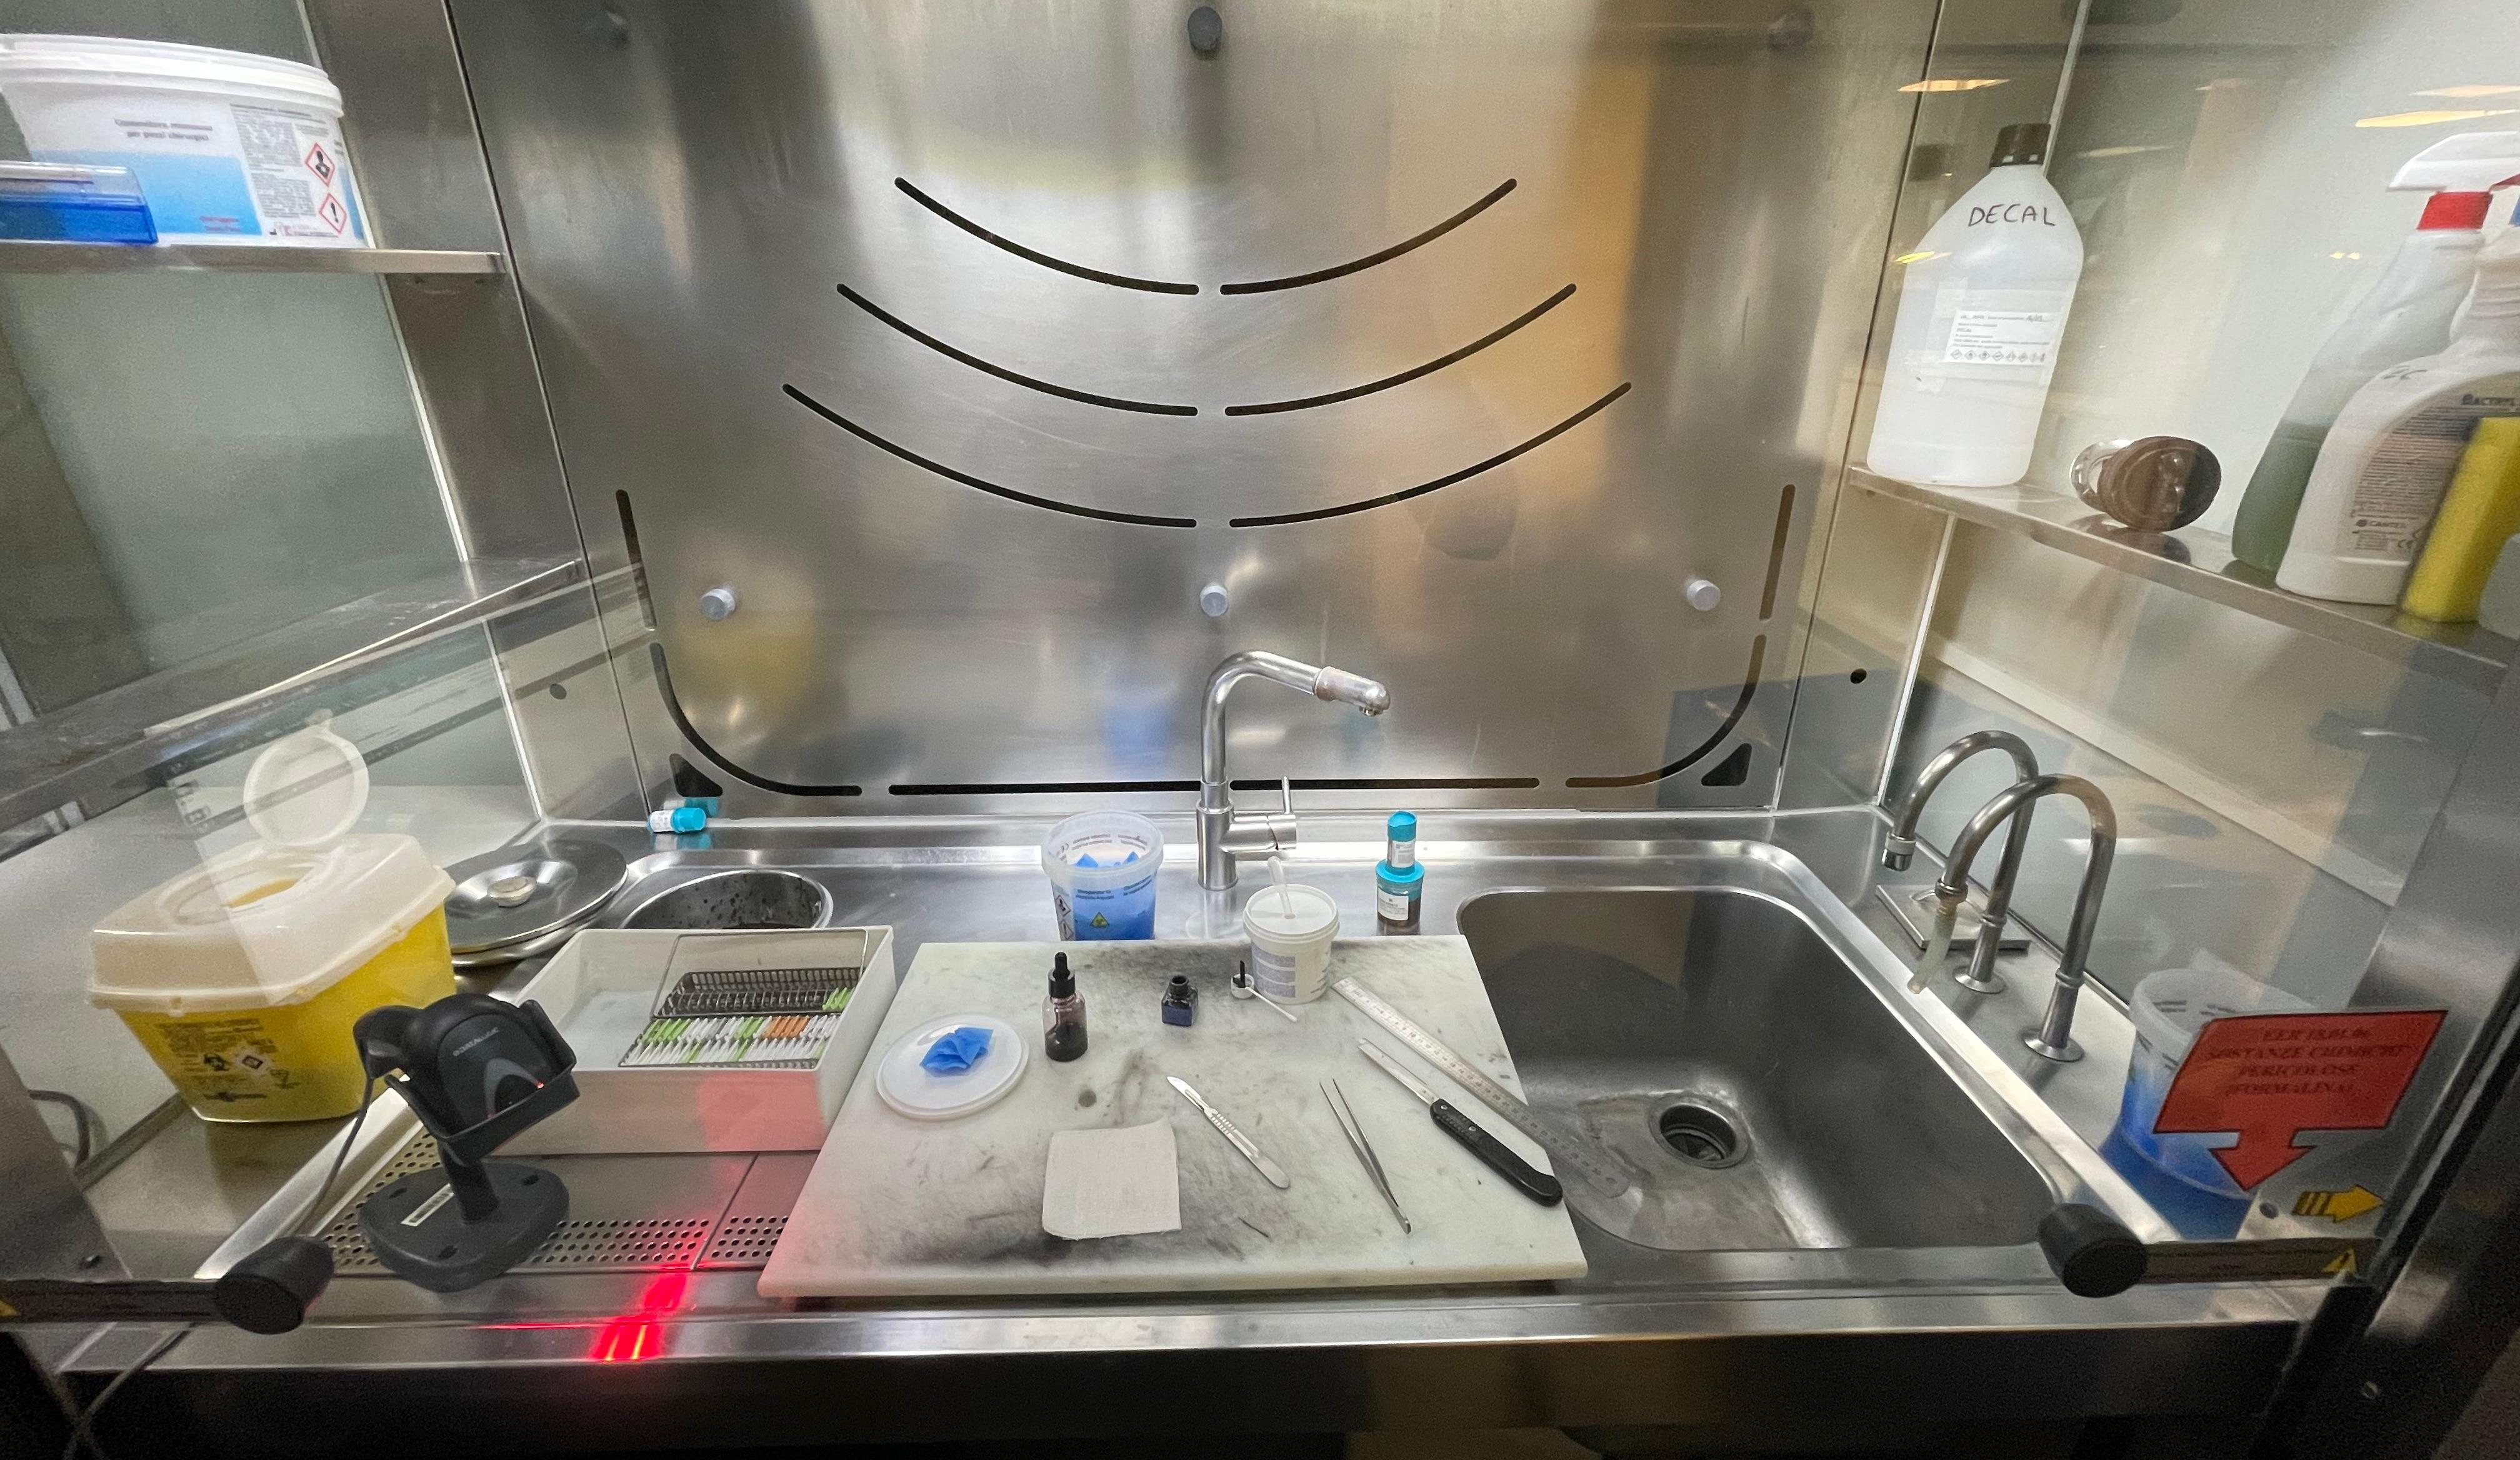
\includegraphics[width=0.85\textwidth]{materiale_campionamento}
    \caption{La postazione di campionamento. Sul tagliere spugnete inumidite con la formalina, ematossilina per marcare i piccoli campioni bioptici, china per marcare i margini chirurgici, acido acetico (barattolo con pipetta) per mordenzare la china, righello, lame, bisturi e pinze per il campionamento. Il lavandino con rubinetto di acqua e formalina  e doccino mobile per il lavaggio della cappa. A sinistra del tagliere il cestello dei blocchetti campionati immerso in adeguata quantità di formalina e un lettore di QRcode per il sistema di tracciabilità.}
    \label{fig:materiale_campionamento}
\end{figure}

\subsection{Stazioni di Lavoro}
Ogni "stazione macroscopica" dovrebbe essere collocata sotto una cappa ben ventilata e contenere i seguenti elementi:
\begin{itemize}
    \item Un tagliere possibilmente inclinato in modo che tutti i fluidi defluiscano direttamente nel lavandino.
    \item Mensole per i contenitori dei campioni.
    \item Accesso immediato a un lavandino con acqua calda e fredda.
    \item Accesso immediato alla formalina.
    \item Attrezzatura per una facile registrazione dell'esame macroscopico (sistemi di dettatura o computer).
    \item Scatola di strumenti, tra cui forbici grandi e piccole, pinze lisce (anatomiche) e dentellate  (chirurgiche) di diverse dimensioni, una sonda (specillo) malleabile, un manico per bisturi, lame monouso, un coltello lungo, un righello e spille per fissare i campioni a una superficie di sughero.
    \item Scatola con cassette e etichette.
\end{itemize}
% 
% \section{Attrezzature Centrali della Sala}
% Oltre alle stazioni di lavoro individuali, la sala macroscopica dovrebbe essere dotata del seguente equipaggiamento centrale:
% \begin{itemize}
%     \item Un grande contenitore di formalina: una configurazione molto conveniente consiste nella sospensione di un grande contenitore dal soffitto, con la formalina pompata in esso tramite una pompa meccanica e il fissativo distribuito nelle singole aree di dissezione tramite un sistema di tubazioni con rubinetti.
%     \item Contenitori con altri fissativi, con istruzioni su come mescolarli al momento dell'uso.
%     \item Strutture fotografiche, idealmente situate in ciascuna stazione per comodità.
%     \item Un'unità radiografica autonoma.
%     \item Un grande frigorifero a 4°C.
%     \item Un piccolo frigorifero a 4°C (ad esempio, per fissativi per microscopia elettronica, pellicole fotografiche, ecc.).
%     \item Sega a nastro - preferibilmente una progettata per l'uso nelle macellerie piuttosto che quelle usate dai carpentieri - situata in uno spazio completamente chiuso e ben ventilato.
%     \item Bilance - una con grande capacità per la maggior parte dei campioni e una bilancia di precisione per campioni più piccoli, come le ghiandole paratiroidi.
%     \item Tagliacarne elettrico commerciale - produce eccellenti sezioni trasversali di campioni solidi per scopi dimostrativi e fotografici.
%     \item Microscopio da dissezione.
%     \item Visualizzatore di radiografie.
%     \item Grande tavolo con lavandino per la dissezione di campioni di grandi dimensioni (come le amputazioni).
%     \item Tavolo centrale per usi multipli (ad esempio, per collocare i contenitori con cassette da inviare al laboratorio di istologia, per mostrare i campioni ai visitatori, per conferenze macroscopiche).
%     \item Strutture per la conservazione dei tessuti e biobanca - include uno spazio per la scrivania, una tavola da taglio coperta da una cappa, un terminale del computer, attrezzature e materiali per il congelamento dei campioni, uno o più congelatori e frigoriferi.
% \end{itemize}

\subsection{Postura durante la dissezione}
Gli operatori in questa area possono scegliere di lavorare seduti o in piedi, a seconda delle preferenze. Idealmente, entrambe le opzioni dovrebbero essere disponibili. Le moderne aree di dissezione sono spesso dotate di scrivanie integrate, alimentazione chiusa di fluidi e fissativi e ventilazione a flusso laminare discendente per proteggere sia il dissezionatore che il personale di supporto dai vapori di formalina.

\subsection{Strumenti di dissezione}
Gli strumenti di dissezione devono essere ergonomicamente accessibili, e la sala deve essere dotata di un'adeguata illuminazione naturale e/o artificiale. I coltelli di grandi dimensioni sono utili per ottenere sezioni trasversali complete di organi come polmoni e fegato, mentre le lame più piccole sono ideali per rifinire i dettagli dei tessuti.

\subsection{Conservazione e gestione dei campioni}
Dopo la dissezione, i tessuti residui devono essere conservati in un'area di archiviazione ventilata e sicura, mentre i materiali di scarto devono essere smaltiti secondo le normative locali sulla salute e sicurezza. Inoltre, prima di fissare i campioni, potrebbe essere necessario riservare una parte del tessuto per l'analisi microbiologica o per altre indagini come la microscopia elettronica o la spettrometria di massa. Alcuni campioni richiedono decalcificazione infine richiedono ulteriori passaggi con soluzioni decalcificanti o cheratolitiche.

\section{Principi Generali per l'Esame Macroscopico}

\subsection{Identificazione e Orientamento del Campione}
È fondamentale che ogni campione sia correttamente identificato e orientato per un'adeguata valutazione patologica. Un campione senza etichetta non dovrebbe mai essere processato. Se il campione arriva in laboratorio senza identificazione, è necessario contattare il medico che ha effettuato la procedura, o in sua assenza, uno degli assistenti per identificare e etichettare correttamente il campione. Ogni campione deve essere accompagnato da un modulo di richiesta di anatomia patologica correttamente compilato, che includa l'identificazione del paziente, età, sesso, dati clinici essenziali, tipo di intervento, reperti chirurgici e il tessuto inviato. Se tali informazioni non sono disponibili, è obbligo del patologo, in quanto consulente medico, esaminare la cartella clinica o, se necessario, vedere il paziente di persona prima di formulare un'opinione.

\subsection{Difficoltà nell'Orientamento del Campione}
Se ci sono difficoltà nell'orientamento del campione, è necessario contattare il chirurgo per richiedere collaborazione nell'identificare la posizione, i punti di riferimento anatomici, i margini chirurgici e altre strutture rilevanti. È importante esaminare con cura tutto il materiale inviato, anche sotto la copertura del contenitore per evitare di perdere frammenti di tessuto.

\subsection{Manipolazione del Campione}
Il campione, specialmente se piccolo, deve essere manipolato su una tavola da taglio pulita utilizzando strumenti puliti. Il problema della contaminazione con frammenti di altri campioni (detto "floater" o metastasi da tagliere) rappresenta una delle principali catastrofi in un laboratorio patologico, poiché può portare a errori irreparabili.

\subsection{Importanza della Conoscenza Anatomica del Patologo}
Anche se il patologo non è un chirurgo o un anatomista, dovrebbe possedere una conoscenza di base dell'anatomia normale, dell'estensione della maggior parte degli interventi chirurgici e delle strutture che ci si aspetta di trovare in una data procedura. La prima fase consiste nell'ispezionare il campione, identificando tutte le componenti normali e anormali. Il patologo dovrebbe quindi posizionare il campione in modo anatomico sulla tavola da taglio e registrare informazioni come tipo di campione, strutture incluse, dimensioni, peso, forma e colore.

\subsection{Margini Chirurgici e Diagnosi Istologica}
Nel caso di margini chirurgici coinvolti da tumori, è cruciale determinare dove si trovino tali margini. Questo richiede un lavoro meticoloso e talvolta noioso, ma è sempre gratificante per la precisione diagnostica. Prima di iniziare la dissezione del campione, si dovrebbe considerare la possibilità di fare fotografie macroscopiche per documentazione.

\subsection{Dissezione del Campione Chirurgico}
Durante la dissezione di un campione chirurgico possono presentarsi tre situazioni: (1) separazione dei componenti principali mentre il campione è fresco; (2) rimozione solo di alcune parti, come i linfonodi regionali, lasciando intatto il resto del campione; (3) fissazione dell'intero campione in un unico blocco. I campioni più grandi possono richiedere una fissazione più lunga in frigorifero per rallentare il processo autolitico, mentre quelli più piccoli possono essere fissati a temperatura ambiente.

\subsection{Gestione di Campioni con Tessuti Molli e Ossa}
I campioni contenenti sia tessuti molli che ossei devono essere gestiti in modo diverso, a seconda della patologia presente. Una tecnica consiste nel congelare l'intero campione fresco e preparare sezioni parallele con una sega a nastro (Figura \ref{fig:sega}). Un'altra tecnica prevede la dissezione accurata dell'osso, lasciando intatto il tessuto molle.

\begin{figure}[h]
    \centering
    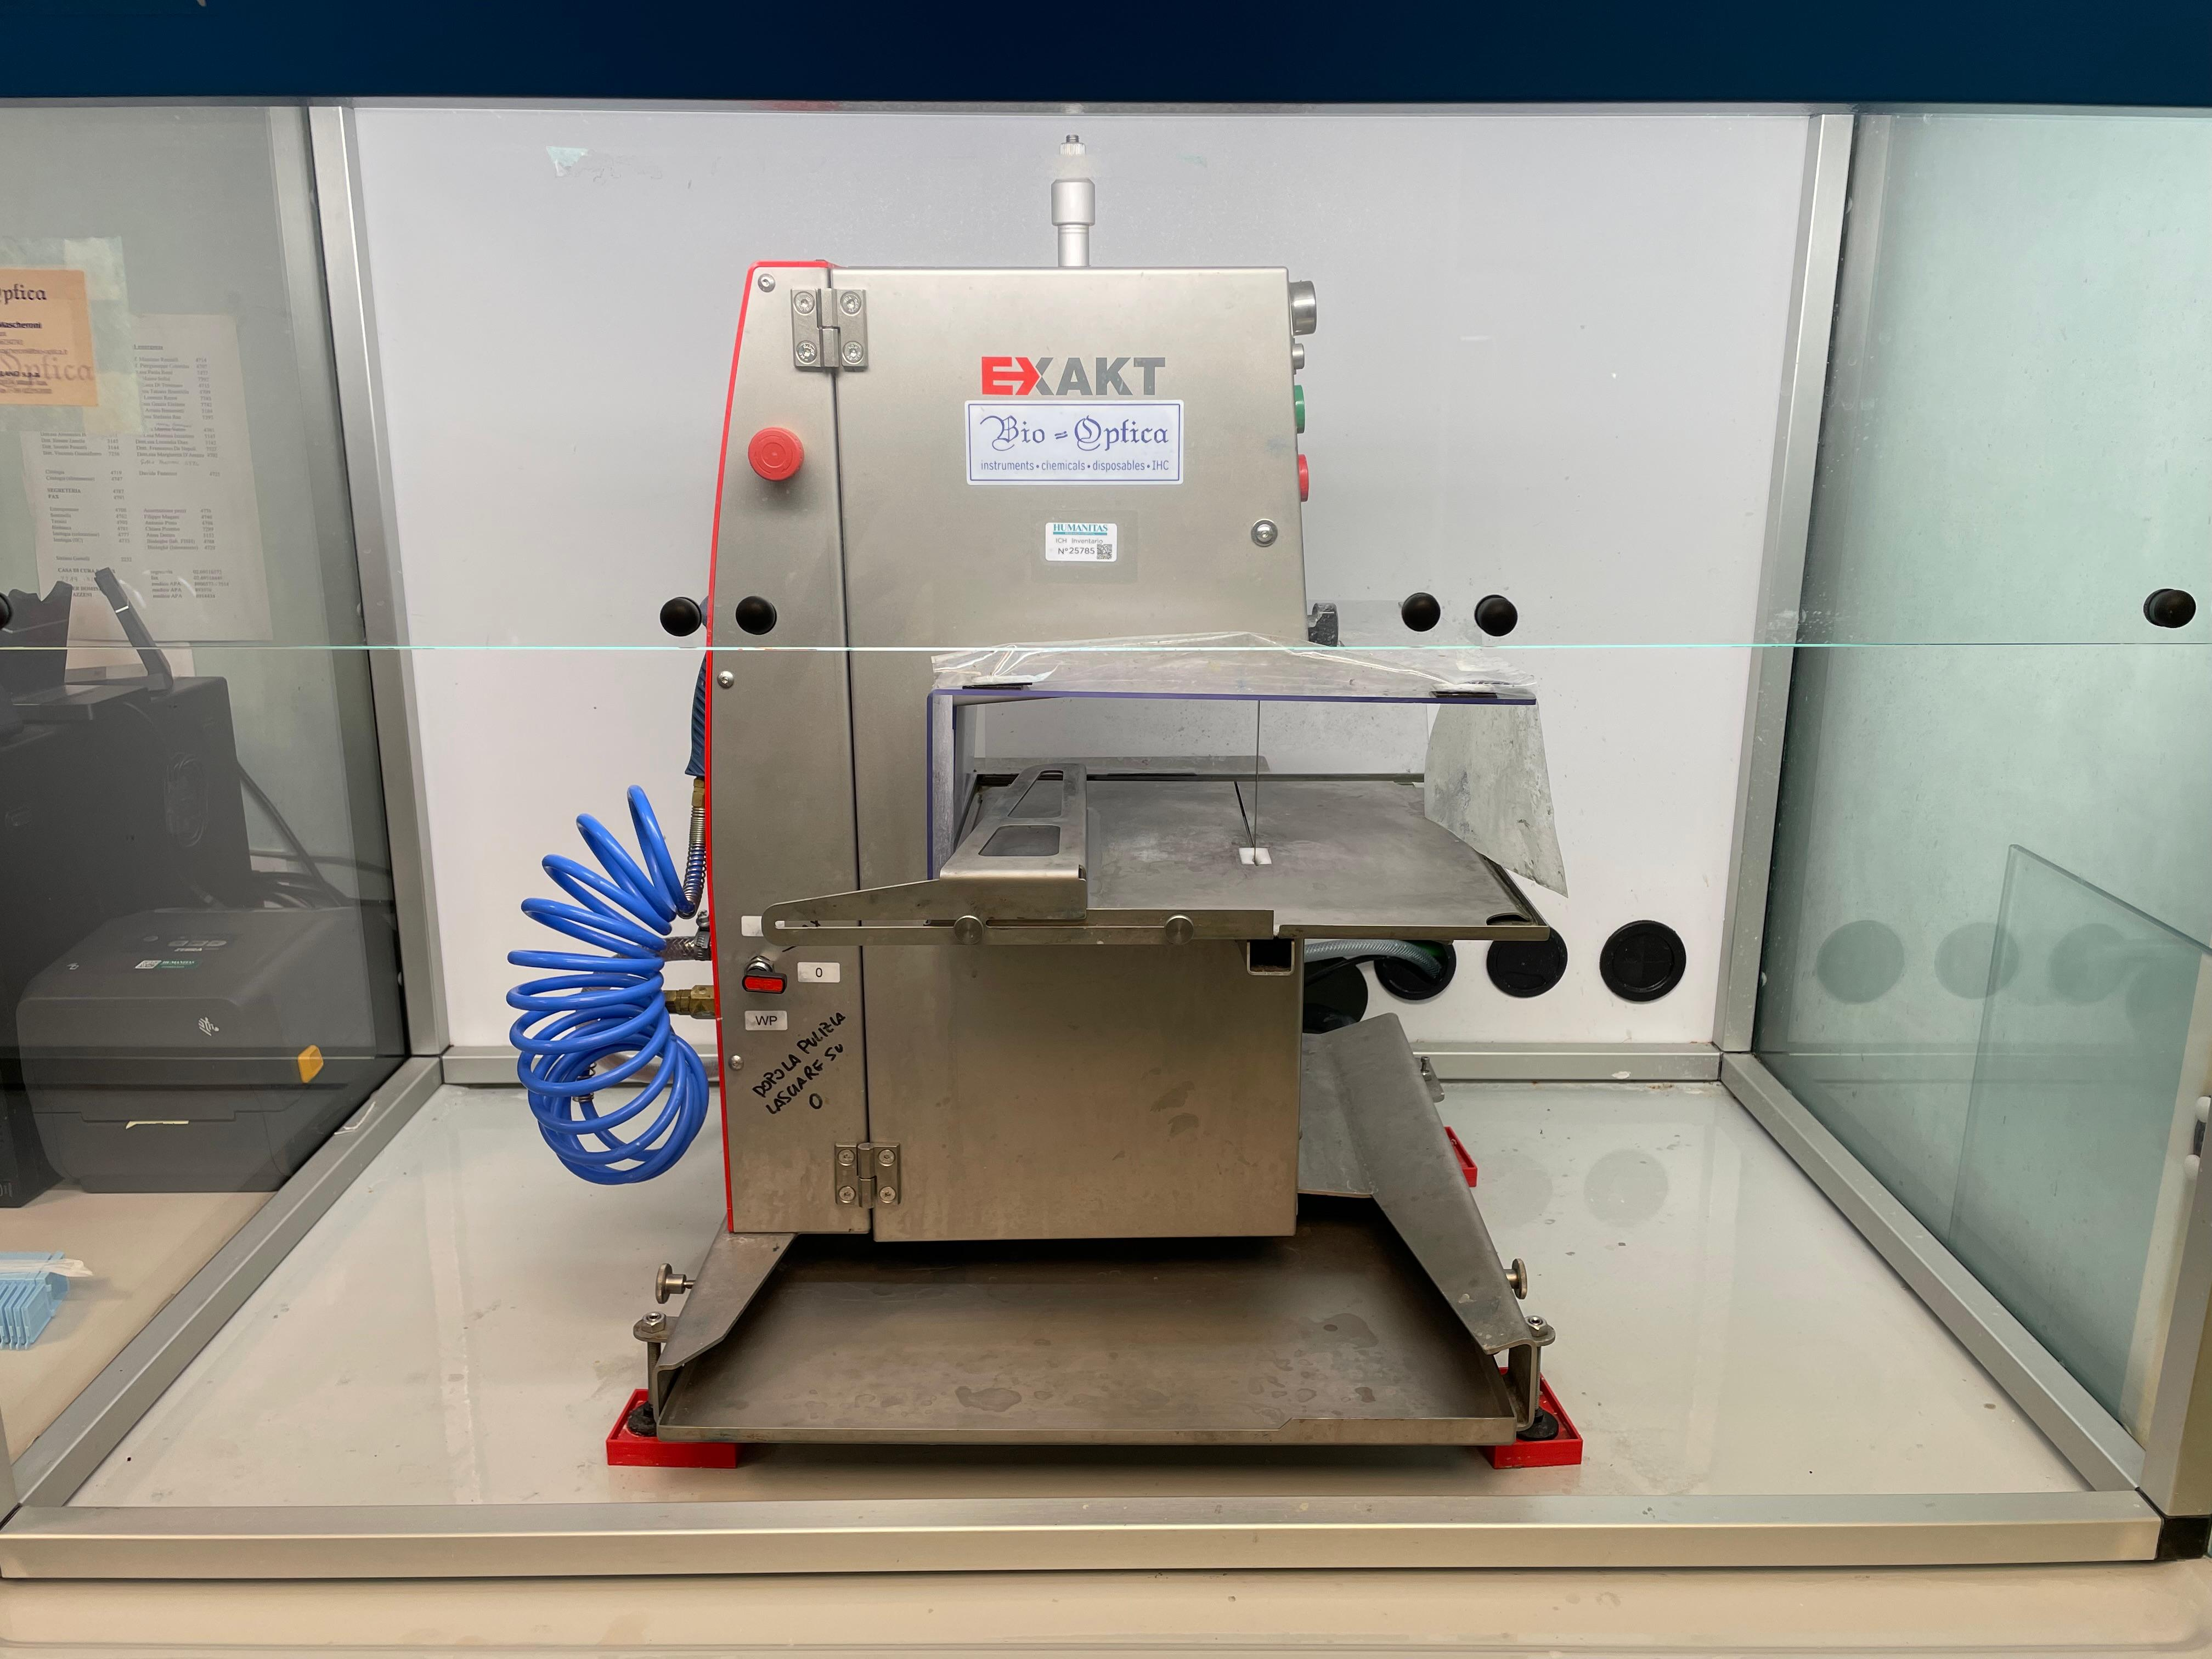
\includegraphics[width=0.85\textwidth]{sega}
    \caption{Sega a nastro per la sezione dei campioni ossei.}
    \label{fig:sega}
\end{figure}

\subsection{Conservazione delle Sezioni e Campioni}
Dopo la dissezione, è consigliabile lasciare intatta una delle migliori sezioni per eventuali fotografie o dimostrazioni macroscopiche. Nessuna parte del campione dovrebbe essere smaltita prima che il caso sia chiuso. È preferibile conservare i tessuti per almeno un mese, ma in alcuni laboratori, lo spazio disponibile può limitare questa pratica.

\subsection{Contaminazione dei Campioni}
La contaminazione dei campioni, conosciuta come "floater", è uno dei problemi più gravi in un laboratorio patologico. Questo può accadere in qualsiasi fase del processo: in sala operatoria, durante la dissezione, l'inclusione in paraffina, la colorazione o il montaggio del vetrino. È essenziale adottare misure per minimizzare questo rischio, anche se non può essere completamente eliminato.

\subsection{Errori di Etichettatura}
Gli errori di etichettatura dei campioni sono un'altra causa importante, anche se rara, di errore medico. La maggior parte degli errori avviene durante la fase di grossing. L'adozione di tecnologie come i codici a barre o i chip a radiofrequenza può ridurre significativamente l'incidenza di tali errori.

\subsection{Riassunto}
L'esame di un campione patologico è un processo complesso che integra l'analisi macroscopica e quella microscopica. Mentre quest'ultima è spesso considerata la più affascinante e gratificante per la sua precisione, non si può sottovalutare l'importanza dell'analisi macroscopica, che offre informazioni cruciali sulla dimensione, la forma e la natura del processo patologico. In effetti, per alcuni campioni, come le valvole cardiache, una dettagliata osservazione macroscopica può rivelarsi molto più informativa rispetto a una semplice sezione microscopica. Un’analisi macroscopica accurata non solo arricchisce la comprensione del caso, ma può anche prevenire errori di interpretazione che potrebbero derivare da una dissezione inadeguata.

La fase di dissezione, insieme alla descrizione macroscopica e alla selezione delle sezioni per lo studio microscopico, riveste un ruolo cruciale nel percorso diagnostico. Se la descrizione macroscopica non viene eseguita con attenzione, si rischia di perdere informazioni vitali che non possono più essere recuperate in seguito. Questa consapevolezza è particolarmente importante quando si trattano campioni complessi, per i quali è fondamentale avere un’adeguata esperienza e conoscenza. Tuttavia, si osserva una certa riluttanza tra i medici in formazione nel cercare il supporto di membri più esperti del personale per l'analisi di campioni difficili, nonostante la stessa ansia non si presenti nel caso delle sezioni microscopiche. Questa situazione è disdicevole, poiché la difficoltà nell'interpretazione di un vetrino può derivare proprio da una fase di campionamento macroscopico insufficiente.

Per garantire un’analisi accurata, è fondamentale che il laboratorio di anatomia patologica sia situato vicino alla sala operatoria. Questo consente ai campioni di essere trasferiti rapidamente in uno stato fresco, riducendo il rischio di deterioramento. I campioni, tranne che per le piccole biopsie, dovrebbero essere portati in sacchetti di plastica per evitare contaminazioni. Nel caso di biopsie di piccole dimensioni, è essenziale immergerle immediatamente in un fissativo appropriato, mentre per campioni di dimensioni maggiori, è consigliabile sigillarli in sacchetti sotto vuoto per un trasporto sicuro, sebbene questo possa creare l'erronea impressione che il campione stia già fissandosi.

La preparazione di un campione per l'analisi istologica non si limita al semplice taglio delle sezioni; ci sono numerosi passaggi da seguire, e il laboratorio deve essere dotato di personale adeguatamente formato per gestire i campioni in modo efficace. La sala di accettazione, dove i campioni vengono ricevuti, deve essere un ambiente ben organizzato e attrezzato per garantire la sicurezza e l’integrità dei campioni stessi. Qui, ogni campione deve essere identificato con un codice unico e confrontato con la documentazione clinica per verificare la sua provenienza. È consigliabile seguire rigide procedure di controllo, coinvolgendo più operatori per garantire l’accuratezza dei dettagli del campione.

Non meno importante è la valutazione iniziale dei campioni, che deve essere effettuata rapidamente in base alle informazioni cliniche e alle osservazioni macroscopiche. Questo primo esame consente di decidere se sono necessari ulteriori studi, come le sezioni congelate o esami specializzati. Inoltre, esistono diverse procedure speciali che possono essere necessarie a seconda delle caratteristiche del campione, come colture batteriche o tecniche di microscopia elettronica. L’impiego di assistenti del patologo ben addestrati può rivelarsi estremamente vantaggioso, poiché possono gestire compiti tecnici sotto la supervisione del patologo, contribuendo a garantire la coerenza e la qualità dei risultati.

La sala di dissezione deve essere un ambiente ben illuminato e ventilato, equipaggiato con strumenti ergonomici e attrezzature di sicurezza. Le dimensioni della sala dovrebbero consentire il lavoro simultaneo di più patologi, con stazioni di lavoro ben attrezzate che includano lavandini, accesso ai fissativi e spazi per la registrazione dei dati. È essenziale che il personale mantenga una postura corretta durante la dissezione per evitare affaticamenti e infortuni.

Ogni campione deve essere manipolato con attenzione per evitare contaminazioni. Anche il più piccolo frammento può compromettere l’analisi, rendendo cruciale mantenere l'integrità del campione in ogni fase del processo. La conoscenza anatomica di base è fondamentale per i patologi, poiché consente di identificare correttamente le strutture e i tessuti durante l’esame macroscopico. È importante esaminare attentamente tutti i campioni, annotando le dimensioni, il colore e altre caratteristiche rilevanti.

Nella gestione dei campioni che includono tessuti molli e ossei, le tecniche di dissezione devono essere adattate alle specifiche necessità patologiche, e i campioni devono essere conservati in modo appropriato dopo la dissezione, evitando di smaltire alcuna parte prima di chiudere il caso. Infine, la riduzione al minimo della contaminazione e degli errori di etichettatura è fondamentale. L'implementazione di tecnologie moderne, come i codici a barre, può significativamente ridurre gli errori e migliorare l'affidabilità del processo diagnostico.